%!TEX root = ../sbc-template.tex

\begin{table}[H]
	\scalefont{0.8}
	\centering
	\caption{Exemplos de funções de ativação}
	\label{tab:ativacoes}
	\begin{adjustbox}{width=1\textwidth}
		\begin{tabular}{l l p{6.5cm} l}
			\toprule
			Nome 			 		& Gráfico & Equação & Intervalo\\
			\midrule
			Identidade ou Linear		&
			 	\Centerstack{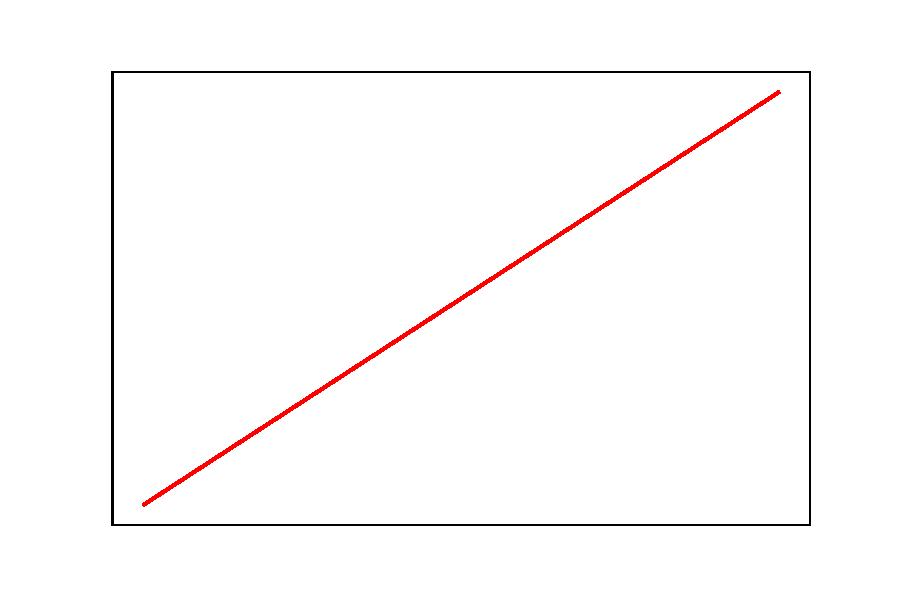
\includegraphics[width=0.15\textwidth]{img/identidade}}
			&
				$
					\begin{aligned}
						\sigma(z) = z
					\end{aligned}
				$
				& $(-\infty, + \infty) $\\
			\hline
			Tangente Hiperbólica		&
				\Centerstack{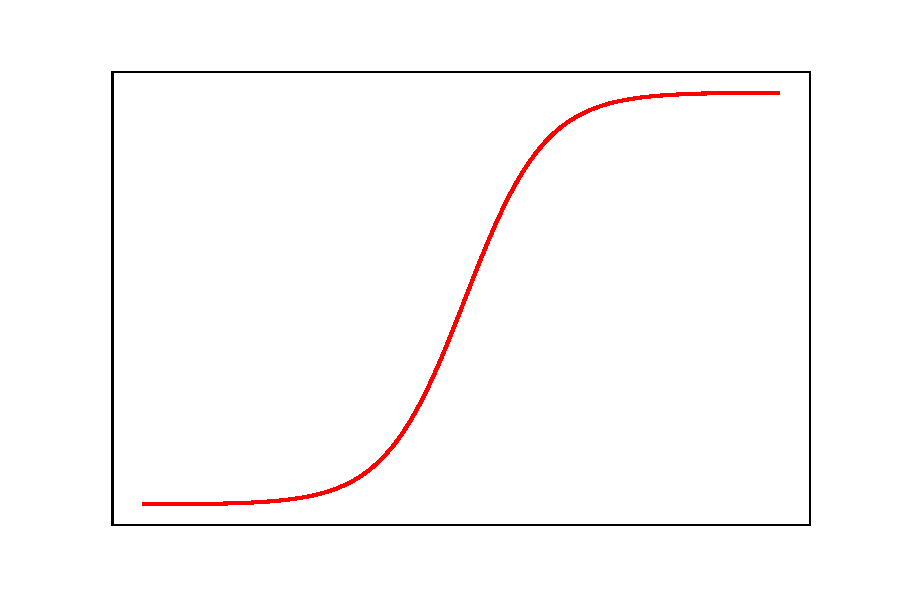
\includegraphics[width=0.15\textwidth]{img/tanh}}
				&
				$
					\begin{aligned}
						\sigma(z) = tanh(z) =\frac{(e^z - e^{-z})}{(e^z + e^{-z})}
					\end{aligned}
				$
				 & $(-1,1)$\\
			\hline
			Sigmoide ou Logística		&
				\Centerstack{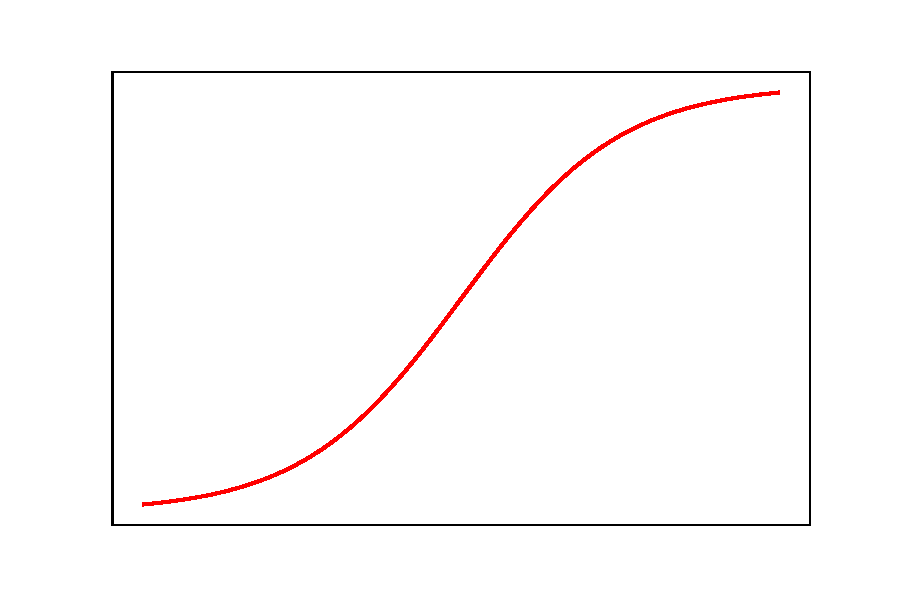
\includegraphics[width=0.15\textwidth]{img/sigmoid}}
				&
				$
					\begin{aligned}
						\sigma(z) = \frac{1}{1+e^{-x}}
					\end{aligned}
				$
				& $ (0,1) $\\
			\hline
			Unidade Linear Retificada	&
				\Centerstack{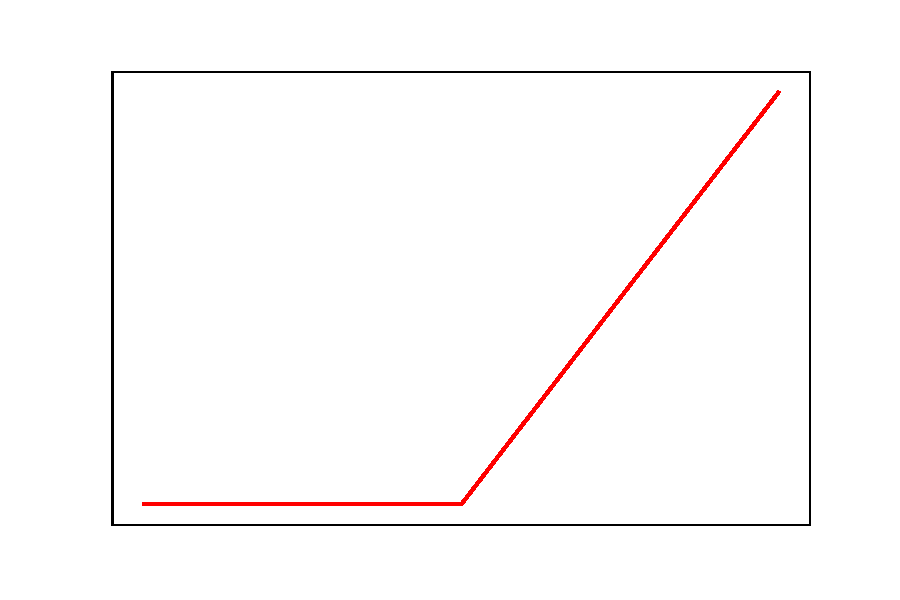
\includegraphics[width=0.15\textwidth]{img/relu}}
				&
				$
					\begin{aligned}
						\sigma(z) = max(0,z)
					\end{aligned}
				$
				& $ [0, \infty) $\\
			\hline
			Softmax					&
				\Centerstack{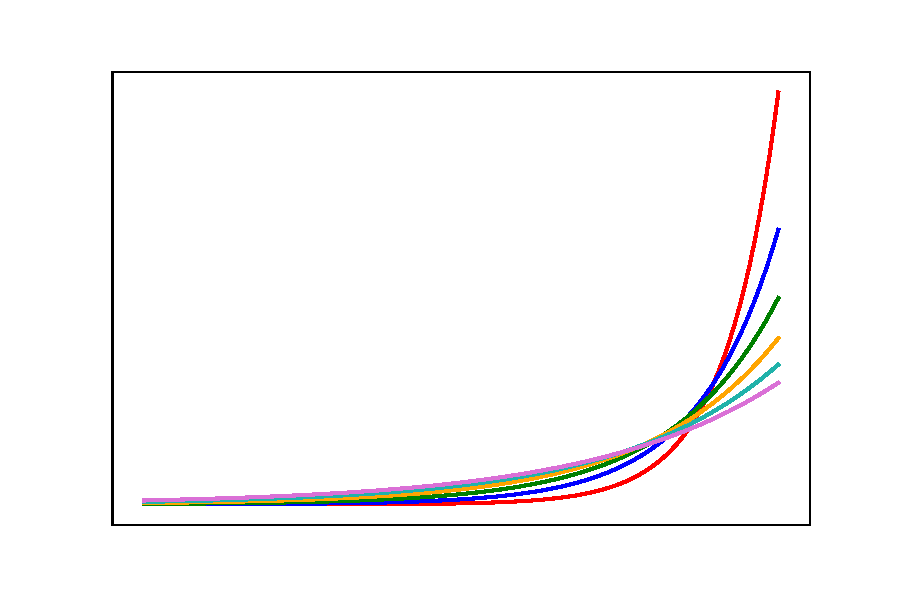
\includegraphics[width=0.15\textwidth]{img/softmax}}
				&
				$
					\begin{aligned}
						g(z_j) = \frac{e^{z_j}}{\sum^K_{j=1} e^{z_k}} \hspace{0.2cm}j=1, \ldots, K
					\end{aligned}
				$
				& $(-\infty, \infty)$\\
			\bottomrule
		\end{tabular}
	\end{adjustbox}
\end{table}
